% !TeX program = lualatex
% !TeX encoding = utf8
% !TeX spellcheck = uk_UA

\documentclass[]{beamer}
\usetheme{PlasmaPhysics}
\usepackage{PlasmaPhysics}
\usepackage{mathtools}
\setlength{\abovedisplayskip}{3pt}
\setlength{\belowdisplayskip}{3pt}
\usetikzlibrary{decorations.pathreplacing}
\newtcolorbox{mysidebyside}[1][]{
    notitle, sidebyside, blanker,
    sidebyside align=center seam,
    halign=center,
    lefthand width=.5\textwidth,
    #1
}



\graphicspath{{pictures/}}
\title[Лекції з фізики плазми]{\bfseries\huge Рух заряджених частинок в плазмі}
\subtitle{\bfseries Лекції з фізики плазми}
\author{Пономаренко С. М.}
\date{}
% https://www.youtube.com/watch?v=zv9Y7YmHyBk
\def\stext#1{\text{
        \makebox[0pt]{
            \tikz[baseline] {\node[text width=50pt, align=center, execute at begin node=\setlength{\baselineskip}{-0.5ex}, blue] {#1};}
        }
}}


\begin{document}




%===============================================================================
\usebackgroundtemplate{
	\tikz\node[opacity=0.1]{\includegraphics[width=\paperwidth,height=\paperheight]{background}};%
}


\begin{frame}
	\thispagestyle{empty}
	\titlepage
\end{frame}





%% --------------------------------------------------------
\section{Вступ}
%% --------------------------------------------------------





% ============================== Слайд ## ===================================
\begin{frame}{Епіграф}{}
	\begin{block}{\textcopyright\ Chen F.~F. Introduction to Plasma Physics and Controlled Fusion}\justifying\itshape
		Плазма у деяких випадках поводиться як рідина, а в деяких --- як скупчення окремих частинок. І перший крок, для того щоб зрозуміти, як мати справу з цією \emph{навіженою особою}, --- це \alert{вивчити поведінку окремих частинок в електричних і магнітних полях}. \\
	\end{block}
\end{frame}
% ===========================================================================




%% --------------------------------------------------------
\section{Дрейфове наближення}
%% --------------------------------------------------------





% ============================== Слайд ## ===================================
\begin{frame}{Дрейфове наближення}{}
	\begin{overprint}
		\onslide<1>
		\begin{itemize}\justifying
			\item Якщо на \alert{ідеальну плазму} діють \alert{сильні зовнішні поля}, то наближено можна \alert{нехтувати внутрішніми полями}, що створюються частинками плазми.
			\item  У цьому наближенні, плазма розглядається як \emph{система незалежних заряджених частинок}, що рухаються по своїх траєкторіях у заданих зовнішніх полях.
		\end{itemize}
		\begin{alertblock}{}\centering
			Єдиним внутрішнім полем, яким ніколи не можна нехтувати, є \alert{електричне поле поляризації}, що виникає внаслідок розподілу зарядів і забезпечує квазінейтральність плазми.
		\end{alertblock}
		\onslide<2>
		Рівняння руху зарядженої частинки в заданих
		зовнішніх полях має вигляд:
		\begin{equation*}
			\tcbhighmath{%
				m \frac{d\vec{v}}{dt} = \frac{Ze}{c}\left[\vec{v}\times\vec{B}\right] + \vec{F},}
		\end{equation*}
		\begin{itemize}
			\item \alert{В загальному вигляді рівняння не можна розв'язати} в аналітичному вигляді, крім найпростіших випадків.
			\item Важливе значення у фізиці плазми має наближений метод його розв'язання, який носить назву \alert{дрейфового наближення}.
		\end{itemize}
	\end{overprint}
\end{frame}
% ===========================================================================




%% --------------------------------------------------------
\section{Рух в однорідному магнітному полі}
%% --------------------------------------------------------






% ============================== Слайд ## ===================================
\begin{frame}{Рух в однорідному магнітному полі}{Циклотронне обертання}
	\begin{onlyenv}<1>
		\begin{columns}
			\begin{column}{0.3\linewidth}
				\tdplotsetmaincoords{65}{125}
    \begin{tikzpicture}[
    >=latex,
    declare function = {
        R = 1;
        w=1;
        v=0.2;
        x(\t)=R*sin(w*\t r);
        y(\t)=R*cos(w*\t r);
        z(\t)=v*\t;
    },
    tdplot_main_coords]
        \coordinate (O) at (0,0,0);
        \coordinate (z) at (0,0,3);
     		\coordinate (x) at (2,00);
      		\coordinate (y) at (0,2,0);

       \draw[->] (O) -- (z) node[anchor=south] {$z$};
       \draw[->] (O) -- (x) node[anchor=south] {$x$};
       \draw[->] (O) -- (y) node[anchor=south] {$y$};

       \draw[blue, thick, variable=\t, domain=0:6.1*pi, samples=150, ->] plot ({x(\t)}, {y(\t)}, {z(\t)});

       \def\k{2.55*pi}
       \draw[canvas is xy plane at z={z(\k)}, dashed, fill=orange!50, opacity=0.5] (0,0) circle (R);

       \node[circle, ball color=blue, inner sep=0pt, font=\tiny, text=white] (T) at ({x(\k)}, {y(\k)}, {z(\k)}) {$+$};

       \draw[->, red] (T) -- ++({y(\k)}, {-x(\k)}, {0}) coordinate (A) node[below, text=black, font=\tiny] {$\vec{v}_\perp$};

       \draw[->, red] (T) -- ++({y(\k)}, {-x(\k)}, {0.3}) coordinate (B) node[above, text=black, font=\tiny] {$\vec{v}$};

       \draw[->, red] (T) -- ++(0, 0, 0.3) coordinate (C) node[above right=-5pt, text=black, font=\tiny] {$\vec{v}_\parallel$};

       \draw[densely dashed] (A) -- (B) -- (C);

       \draw[canvas is xy plane at z={z(\k)}, ->, blue] (0,0) -- (T) node[above=-2pt, font=\tiny, pos=0.3] {$\vec\rho$};

    \end{tikzpicture}
			\end{column}
			\begin{column}{0.7\linewidth}\small
				Рівняння руху:
				\begin{equation*}
					m \frac{d\vec{v}}{dt} = \frac{Ze}{c}\left[\vec{v}\times\vec{B}\right].
				\end{equation*}
				Складові вектора швидкості:
				$
					\vec{v} = \vec{v}_\perp + \vec{v}_\parallel
				$
				\begin{align*}
					\dot{\vec{v}}_\parallel & = 0                                                                                                      \\
					\dot{\vec{v}}_\perp     & =  \left[-\frac{Ze\vec{B}}{mc}\times\vec{v}_\perp\right] = \left[\vec{\Omega}\times\vec{v}_\perp\right].
				\end{align*}
			\end{column}
		\end{columns}
	\end{onlyenv}
	\begin{onlyenv}<1->
		\begin{block}{Циклотронна частота}
			\begin{equation*}
				\tcbhighmath{%
					\vec\Omega = -\frac{Ze\vec{B}}{mc}
				}\quad \Omega = \frac{ZeB}{mc}\ \text{(не модуль)}.
			\end{equation*}
		\end{block}
	\end{onlyenv}
	\begin{onlyenv}<2>
		\begin{columns}
			\begin{column}{0.5\linewidth}\centering
				    \begin{tikzpicture}
        \draw [blue, domain=0:2*pi,variable=\t, samples=55,
        thick,
        decoration={
            markings,
            mark=at position 0.5 with {\arrow[xshift=0pt]{latex}},
            },
            postaction={decorate}
            ]
            plot[] ({sin(\t r)}, {cos(\t r)});
            \coordinate (start) at ({sin(0.5*pi r)}, {cos(0.5*pi r)});
            \node[circle, ball color=blue, inner sep=0, text=white] at (start) {$+$};

            \begin{scope}[shift={(2,0)}]
            \draw [red,
            thick,
            domain=0:2*pi,variable=\t, samples=55,
            decoration={
            markings,
            mark=at position 0.5 with {\arrow[xshift=2pt, scale=0.75]{latex}},
            },
            postaction={decorate}
            ]
            plot[] ({-0.5*sin(\t r)}, {0.5*cos(\t r)});
            \coordinate (start) at ({-0.5*sin(0.5*pi r)}, {0.5*cos(0.5*pi r)});
            \node[circle, ball color=red, inner sep=0.5pt, text=white, font=\tiny] at (start) {\tikz\draw (0,0) -- ++(0.1, 0);};
            \end{scope}

            \coordinate(A) at (1,1);
            \draw[<->, gray] (0,0) -- (A) node[right, font=\scriptsize, text=gray] {Ведучий центр} -- (2,0) ;

            \begin{scope}[blue, shift={(1,1.5)}]
            \fill (0,0) circle (0.05);
            \draw (0,0) circle (0.1) node[right] {$\vec{B}$};
            \end{scope}
    \end{tikzpicture}
			\end{column}
			\begin{column}{0.5\linewidth}\centering
				\tdplotsetmaincoords{60}{0}
\begin{tikzpicture}[>=latex, tdplot_main_coords]
	\tdplotsetrotatedcoords{0}{20}{0}
    % -------------- ion -----------------
	\begin{scope}[tdplot_rotated_coords]
		\coordinate (O) at (0,0,0);
		\coordinate (z) at (0,0,1.5);
		\coordinate (x) at (1,00);
		\coordinate (y) at (0,1,0);
		\coordinate (-z) at (0,0,-1.5);

		%    \draw[->] (O) -- (y) node[anchor=south] {$y$};
		%    \draw[->] (O) -- (x) node[anchor=south] {$x$};

		\draw[->, gray, thick] (O) -- (z) node[anchor=south] {$\vec{B}$};
		\draw[->, blue, thick] (O) -- (-z) node[anchor=north] {$\vec\Omega$};
		\draw[canvas is xy plane at z=0,
			draw=blue,
            thick,
			decoration={markings,
					mark=at position 0.75 with {\arrow[rotate=180, xshift=2pt]{latex}},
				},
			postaction=decorate,
		] (0,0) ++(90 :1) arc [start angle=90, delta angle=335, radius=1];

		\begin{scope}[canvas is xy plane at z=0]
            \node[circle, fill=blue, inner sep=1pt] at (0,0) {};
			\node[transform shape=false, ball color=blue, circle, inner sep=0, text=white] at (45:1) {$+$};
		\end{scope}

        % -------------- electron -----------------
		\begin{scope}[xshift=3cm]
			\coordinate (O) at (0,0,0);
			\coordinate (z) at (0,0,1.5);
			\coordinate (x) at (1,00);
			\coordinate (y) at (0,1,0);
			\coordinate (w) at (0,0,1.25);

			%    \draw[->] (O) -- (y) node[anchor=south] {$y$};
			%    \draw[->] (O) -- (x) node[anchor=south] {$x$};

			\draw[->, gray, thick] (O) -- (z) node[anchor=south] {$\vec{B}$};
			\draw[->, red, thick] (O) -- (w) node[anchor=west] {$\vec\Omega$};
			\draw[canvas is xy plane at z=0,
				draw=red,
                thick,
				decoration={markings,
						mark=at position 0.2 with {\arrow[xshift=2pt]{latex}},
					},
				postaction=decorate,
			] (0,0) ++(90 :1) arc [start angle=90, delta angle=335, radius=1];

			\begin{scope}[canvas is xy plane at z=0]
                \node[circle, fill=blue, inner sep=1pt] at (0,0) {};
				\node[transform shape=false, ball color=red, circle, inner sep=1pt, text=white] at (105:1) {\tikz\draw[]  (0,0) -- ++(0.1,0);};
			\end{scope}
		\end{scope}
	\end{scope}
\end{tikzpicture}
			\end{column}
		\end{columns}
		\begin{block}{Ларморовий радіус}
			\begin{equation*}
				\rho = \frac{v_\perp}{\Omega} = \frac{mcv_\perp}{ZeB}.
			\end{equation*}
		\end{block}
	\end{onlyenv}
\end{frame}
% ===========================================================================




%% --------------------------------------------------------
\section{Види дрейфу}
%% --------------------------------------------------------





% ============================== Слайд ## ===================================
\begin{frame}{Види дрейфу}{}
	\begin{block}{}
		Якщо сила $\vec{F}$ у рівнянні відсутня і магнітне
		поле однорідне, то рух частинки являє собою поєднання циклотронного обертання і руху вздовж силової лінії.
	\end{block}
	Якщо  $\vec{F} \neq 0$ на цю найпростішу картину накладаються різні види дрейфового руху:
	\begin{enumerate}
		\item \alert{Електричний дрейф}: рух під дією сили з боку постійного електричного поля.
		\item \alert{Гравітаційний дрейф}: рух під дією сили тяжіння.
		\item \alert{Градієнтний дрейф}: рух в неоднорідному магнітному полі $\vec{B}$, що змінюється за величиною.
		\item \alert{Відцентровий дрейф}:  рух в неоднорідному магнітному полі $\vec{B}$, що змінюється за напрямком.
		\item \alert{Поляризаційний дрейф}: рух у змінному за часом електричному полі.
	\end{enumerate}
\end{frame}
% ===========================================================================




%% --------------------------------------------------------
\section{Кількісний розгляд дрейфового руху}
%% --------------------------------------------------------




% ============================== Слайд ## ===================================
\begin{frame}{Кількісний розгляд дрейфового руху}{}\small
	\begin{onlyenv}<1>
		\begin{columns}
			\begin{column}{0.17\linewidth}
				\begin{center}
					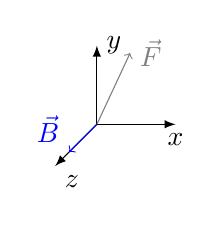
\begin{tikzpicture}[]
    \draw[-latex] (0, 0) -- ++(0, 1) node[right] {$y$};
    \draw[->, gray] (0, 0) -- ++(65: 1)  node[right, text=gray] {$\vec{F}$};
    \draw[-latex] (0, 0) -- ++(1, 0) node[below] {$x$};
    \draw[-latex] (0, 0) -- ++(-135:0.75) node[below right] {$z$};
    \draw[->, blue] (0, 0) -- ++(-135:0.5) node[above left, text=blue] {$\vec{B}$};
\end{tikzpicture}
				\end{center}
			\end{column}
			\begin{column}{0.83\linewidth}\small
				Рівняння руху:
				\begin{equation*}
					\begin{dcases}
						\frac{dv_x}{dt} & = \Omega v_y + \frac{F_x}{m}   \\
						\frac{dv_y}{dt} & = -\Omega v_x + \frac{F_y}{m}.
					\end{dcases}
				\end{equation*}
			\end{column}
		\end{columns}
	\end{onlyenv}
	\begin{onlyenv}<1-2>
		Комплексний вигляд рівнянь руху:
		\begin{equation*}
			\frac{d}{dt}(v_x + iv_y) = -i\Omega(v_x + iv_y) + \frac{F_x + iF_y}{m}.
		\end{equation*}
		Розв'язок:
		\begin{equation*}
			v_x + iv_y = Ce^{-i(\Omega t + \phi_0)} + \frac{F_y}{m\Omega} - i\frac{F_x}{m\Omega}.
		\end{equation*}
		\begin{equation*}
			v_x = v_\perp\cos(\Omega t + \phi_0) + \frac{F_y}{m\Omega},\quad
			v_y = - v_\perp\sin(\Omega t + \phi_0) - \frac{F_x}{m\Omega}
		\end{equation*}
	\end{onlyenv}
	\begin{onlyenv}<2>
		\begin{align*}
			x &= x_0 +  \frac{v_\perp}{\Omega}\sin(\Omega t + \phi_0) + \frac{F_y}{m\Omega} t, \\
			y &= y_0 + \frac{v_\perp}{\Omega}\cos(\Omega t + \phi_0) - \frac{F_x}{m\Omega} t,
		\end{align*}
        де $(x_0, y_0)$ --- координати ведучого центу.
	\end{onlyenv}
	\begin{onlyenv}<3>
		\begin{block}{Швидкість дрейфу}
			Усереднену за період $T = \frac{2\pi}{\Omega}$ швидкість руху заряду називають \alert{швидкістю дрейфу}.
		\end{block}
		\begin{equation*}
			\avg{v_x} = v^F_x = \frac{\avg{F_y}}{m\Omega} =  \frac{c}{Ze} \frac{\avg{F_y} B_z}{B^2},\quad
			\avg{v}_y = v^F_y = - \frac{\avg{F_x}}{m\Omega} =  - \frac{c}{Ze} \frac{\avg{F_x} B_z}{B^2}.
		\end{equation*}

		\begin{block}{Швидкість дрейфу (векторна форма)}
			\begin{equation*}
				\tcbhighmath{
					\vec{v}_F = \frac{c}{Ze}\frac{\vec{\avg{F}}\times\vec{B}}{B^2}.
				}
			\end{equation*}
		\end{block}
	\end{onlyenv}
\end{frame}
% ===========================================================================





%% --------------------------------------------------------
\section{Електричний дрейф}
%% --------------------------------------------------------




% ============================== Слайд ## ===================================
\begin{frame}{Електричний дрейф}{Рух у схрещених полях $\vec{E}\perp\vec{B}$}
	\begin{overprint}
		\begin{block}{}\justifying
			Якщо $\vec{F} = Ze\vec{E}$ ---  такий дрейф називається \alert{електричним}, або \alert{дрейфом у схрещених полях}.
		\end{block}
		\onslide<1>
		%		\vspace*{-2em}
		\begin{columns}[T]
			\begin{column}{0.17\linewidth}
				\begin{center}
					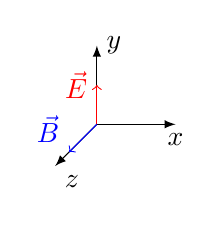
\begin{tikzpicture}[]
    \draw[-latex] (0, 0) -- ++(0, 1) node[right] {$y$};
    \draw[->, red] (0, 0) -- ++(0, 0.5) node[left, text=red] {$\vec{E}$};
    \draw[-latex] (0, 0) -- ++(1, 0) node[below] {$x$};
    \draw[-latex] (0, 0) -- ++(-135:0.75) node[below right] {$z$};
    \draw[->, blue] (0, 0) -- ++(-135:0.5) node[above left, text=blue] {$\vec{B}$};
\end{tikzpicture}
				\end{center}
			\end{column}
			\begin{column}{0.83\linewidth}\small
				\begin{align*}
					v_x & = v_\perp\cos(\Omega t + \phi_0) + \frac{ZeE}{m\Omega}, \\
					v_y & = - v_\perp\sin(\Omega t + \phi_0)
				\end{align*}
				\begin{align*}
					x & = x_0 + \frac{v_\perp}{\Omega}\sin(\Omega t + \phi_0)+ \frac{ZeE}{m\Omega} t, \\
					y & = y_0 + \frac{v_\perp}{\Omega}\cos(\Omega t + \phi_0)
				\end{align*}
			\end{column}
		\end{columns}
		\begin{block}{Швидкість електричного дрейфу}
			\begin{equation*}
				\tcbhighmath{
					\vec{v}_E = c\frac{\vec{E}\times\vec{B}}{B^2}.
				}
			\end{equation*}
		\end{block}
		\onslide<2>
		\begin{center}
			\begin{tikzpicture}[
    declare function={
    w = 1;
    v = 0.5;
    v0 = 1;
    x(\t,\k)=v*\t-v0/(\k*w)*sin((\k*w)*\t r);
    y(\t,\k)=v0/(\k*w)*(1-cos((\k*w)*\t r));
    },
    ]
    \draw[-latex] (0, 0) -- ++(0, 4) node[right] {$y$};
    \draw[->, red] (0, 0) -- ++(0, 2) node[left, text=red] {$\vec{E}$};

    \draw[-latex] (0, 0) -- ++(9, 0) node[below] {$x$};
    \draw[-latex] (0, 0) -- ++(-135:2) node[below right] {$z$};
    \draw[->, blue] (0, 0) -- ++(-135:1) node[above left, text=blue] {$\vec{B}$};

    \draw[-latex] (0, -1.5) -- ++(2,0) node[right] {$\vec{v}_E = c\frac{\vec{E}\times\vec{B}}{B^2}$};

    \draw[blue, thick, domain=0:5*pi, variable=\t, samples=150,
    decoration={
                markings,
                mark=at position 0.05 with {\arrow{latex}},
                mark=at position 0.85 with {\arrow{latex}},
                },
                postaction={decorate}
    ] plot ({x(\t, 1)}, {y(\t, 1)} );

    \draw[red, thick, domain=0:5*pi, variable=\t, samples=550,
    decoration={
                markings,
                mark=at position 0.05 with {\arrow[xshift=5pt]{latex}},
                mark=at position 0.85 with {\arrow[xshift=5pt]{latex}},
                },
                postaction={decorate}
    ] plot ({x(\t, -3)}, {y(\t, -3)} );
    \begin{scope}[shift={(6,3.5)}]
        \node[draw=red, inner sep=5pt] at (0,0) {%
        \begin{minipage}{4cm}\scriptsize%
            \vspace*{-3ex}
            \begin{align*}
                x &= \frac{eE}{\Omega} t -\frac{v_0}{\Omega}\sin(\Omega t), \\
                y &= \frac{v_0}{\Omega}\left(1 - \cos(\Omega t )\right).
            \end{align*}
        \end{minipage}
        };
    \end{scope}
\end{tikzpicture}
		\end{center}
		\onslide<3>
		\begin{block}{Швидкість електричного дрейфу}\justifying
			\begin{equation*}
				\tcbhighmath{
					\vec{v}_E = c\frac{\vec{E}\times\vec{B}}{B^2}.
				}\qquad |v_E| = c\frac{E}{B}.
			\end{equation*}
		\end{block}
		\begin{block}{}
			Формули застосовні лише за умови, що напруженість електричного поля значно менша за індукцію магнітного поля \alert{$E \ll B$}.

			\medskip

			Швидкість електричного дрейфу не залежить від заряду частинки. Електрони та йони дрейфують при цьому в одному напрямку і з однаковою швидкістю.

			\medskip

			Електричний дрейф не призводить до розділення зарядів, а викликає тільки рух плазми як цілого.
		\end{block}
	\end{overprint}
\end{frame}
% ===========================================================================




%% --------------------------------------------------------
\section{Гравітаційний дрейф}
%% --------------------------------------------------------





% ============================== Слайд ## ===================================
\begin{frame}{Гравітаційний дрейф}{}
	\begin{block}{}\justifying
		Якщо $\vec{F} = m\vec{g}$ ---  такий дрейф називається \alert{гравітаційним}.
	\end{block}
	\begin{block}{Швидкість гравітаційного дрейфу}
		\begin{equation*}
			\vec{v}_g = \frac{1}{\Omega B}\left[\vec{g}\times\vec{B}\right].
		\end{equation*}
	\end{block}
	\begin{block}{}\justifying
		Гравітаційний дрейф схожий на дрейф в електричному полі тим, що
		його напрямок перпендикулярний як прикладеній силі, так і напрямку магнітного поля $\vec{B}$. Швидкість гравітаційного дрейфу має різний напрямок залежно від знака заряду частинки.
	\end{block}
	\begin{alertblock}{}\justifying
		Величина швидкості дрейфу спричиненого звичайною силою тяжіння, здебільшого є нехтувано малою.
	\end{alertblock}

\end{frame}
% ===========================================================================




%% --------------------------------------------------------
\section{Градієнтний дрейф}
%% --------------------------------------------------------




% ============================== Слайд ## ===================================
\begin{frame}{Градієнтний дрейф}{}
	\framesubtitle<1>{Основна ідея}
	\framesubtitle<2-4>{Викладки \ldots}
	\framesubtitle<5>{Аналіз розв'язків}
	\begin{onlyenv}<1>
		\begin{block}{}\justifying
			Якщо магнітне поле постійне в часі, але неоднорідне, причому його напрямок усюди однаковий, а змінюється лише напруженість $ \vec{B} $ через наявність слабкого градієнта $\nabla B$, перпендикулярного напряму $\vec{B}$. При цьому виникає \alert{ градієнтний дрейф}.
		\end{block}
		\begin{center}
			\begin{tikzpicture}[
    declare function = {
    R = 0.5;
    dR = 0.05;
    x(\t)=(1-(R+dR*\t)*cos(\t r));
    y(\t)=(R+dR*\t)*sin(\t r);
    },
]
    \draw[-latex] (0, 0) -- ++(0, 2) node[right] {$y$};
    \draw[-latex] (0, 0) -- ++(4, 0) node[below] {$x$};
    \draw[-latex] (0, 0) -- ++(-135:1.75) node[below right] {$z$};

    \draw[->, blue] (0, 0) -- ++(-135:1.25) node[above left, text=blue] {$\vec{B}$};

    \foreach \y in {1, 1.5, 1.8, 2}{
    \draw[->, blue!80, opacity=0.5] (0, \y) -- ++(-135:1.25);
    }

    \draw[->, gray, thick] (0, 0) -- ++(0, 1.5) node[left, text=gray] {$\vec\nabla B$};


    \draw[blue, samples=100, domain=0:2*pi, variable=\t,
    decoration={
        markings,
        mark=at position 0.85 with {\arrow{latex}},
        },
        postaction={decorate}
    ] plot ( {x(\t)}, {y(\t)});

    \node[circle, ball color=blue, inner sep=0, text=white] at ({x(pi/2)}, {y(pi/2)}) {$+$};

    \draw[thick, -latex] (1,0) -- node[below, font=\scriptsize] {$\vec{v}_{\nabla B}$} ++(-0.5,0);

        \draw[red, samples=100, domain=0:2*pi, variable=\t,
%        xscale=-0.5, yscale=0.5,
        decoration={
            markings,
            mark=at position 0.6 with {\arrow[xshift=2pt]{latex}},
            },
            postaction={decorate}
        ] plot ( {3-0.5*x(\t)}, {0.5*y(\t)});

        \node[circle, ball color=red, inner sep=0.5pt, text=white] at ({3-0.5*x(pi/2)}, {0.5*y(pi/2)}) {\tikz\draw[] (0,0) -- (0.1,0);};

        \draw[thick, -latex] (2.5,0) --  node[anchor=north west, font=\scriptsize] {$\vec{v}_{\nabla B}$} ++(0.5,0);
\end{tikzpicture}
		\end{center}
	\end{onlyenv}
	\begin{onlyenv}<2>\small
		Рівняння руху:
		\begin{equation*}
			\frac{dv_x}{dt} = \frac{ZeB}{mc}v_y, \quad
			\frac{dv_y}{dt} = -\frac{ZeB}{mc} v_x.
		\end{equation*}
		Розв'язки в нульовому наближенні:
		\begin{equation*}
			v_x  = v_\perp\cos(\Omega t + \phi_0),  \quad
			v_y  = - v_\perp\sin(\Omega t + \phi_0)
		\end{equation*}
		\begin{equation*}
			x = x_0 + \frac{v_\perp}{\Omega} \sin(\Omega t + \phi_0), \quad
			y = y_0 + \frac{v_\perp}{\Omega} \cos(\Omega t + \phi_0).
		\end{equation*}
		Магнітне поле:
		\begin{equation*}
			B(y) = B_0 + \frac{\partial B}{\partial y} (y - y_0)
		\end{equation*}
	\end{onlyenv}
	\begin{onlyenv}<3>\small
		Рівняння руху:
		%			\begin{align*}
		%				\frac{dv_x}{dt} & = -\frac{Ze}{mc}v_\perp\sin(\Omega t + \phi_0)\left( B_0 - \frac{v_\perp}{\Omega}\frac{\partial B}{\partial y}  \cos(\Omega t + \phi_0)\right) , \\
		%				%
		%				\frac{dv_y}{dt} & = \frac{Ze}{mc} v_\perp\cos(\Omega t + \phi_0)\left( B(y_0) - \frac{v_\perp}{\Omega}\frac{\partial B}{\partial y} \cos(\Omega t + \phi_0)\right).   \\
		%			\end{align*}
		\begin{align*}
			\frac{dv_x}{dt} & = \frac{Ze}{mc}v_yB_0 + \frac{Ze}{mc}v_y \frac{\partial B}{\partial y} (y - y_0),  \\
			%
			\frac{dv_y}{dt} & = -\frac{Ze}{mc}v_xB_0 - \frac{Ze}{mc}v_x \frac{\partial B}{\partial y} (y - y_0). \\
		\end{align*}
	\end{onlyenv}
	\begin{onlyenv}<3-4>\small
		Розкриваємо дужки:
		\begin{align*}
			\frac{dv_x}{dt} & = \Omega v_y - \frac{v^2_\perp}{B} \frac{\partial B}{\partial y} \sin(\Omega t + \phi_0) \cos(\Omega t + \phi_0) , \\
			\frac{dv_y}{dt} & = -\Omega v_x - \frac{v^2_\perp}{B}\frac{\partial B}{\partial y}   \cos^2(\Omega t + \phi_0).
		\end{align*}
	\end{onlyenv}
	\begin{onlyenv}<4>\small
		Сили за періодом:
		\begin{align*}
			F_x & = - m\Omega \frac{v^2_\perp}{B} \frac{\partial B}{\partial y}  \sin(\Omega t + \phi_0) \cos(\Omega t + \phi_0), \quad   \avg{F_x} = 0                             \\
			F_y & = - m\Omega \frac{v^2_\perp}{B} \frac{\partial B}{\partial y} \cos^2(\Omega t + \phi_0), \quad \avg{F_y} = - \frac{mv^2_\perp}{2B} \frac{\partial B}{\partial y}.
		\end{align*}
		У векторному вигляді
		\begin{equation*}
			\vec{\avg{F}} = - \frac{mv^2_\perp}{2B}\vec\nabla B.
		\end{equation*}
	\end{onlyenv}
	\begin{onlyenv}<5>\small
		\begin{block}{Швидкість градієнтного дрейфу}
			\begin{equation*}
				\vec{v}_{\nabla B} = \frac{c}{Ze}\frac{\vec{\avg{F}}\times\vec{B}}{B^2}, \quad \tcbhighmath{
					\vec{v}_{\nabla B} =  \frac{v^2_\perp}{2\Omega}\frac{[\vec{B}\times\vec{\nabla}B]}{B^2}.
				}
			\end{equation*}
		\end{block}
		Знак $ \Omega $ визначається знаком заряду, тому електрони та йони в неоднорідному магнітному полі дрейфують у протилежних напрямках, що призводить до виникнення електричного струму.
		\begin{center}
			\begin{tikzpicture}[
    declare function = {
    R = 0.5;
    dR = 0.05;
    x(\t)=(1-(R+dR*\t)*cos(\t r));
    y(\t)=(R+dR*\t)*sin(\t r);
    },
]
    \draw[-latex] (0, 0) -- ++(0, 2) node[right] {$y$};
    \draw[-latex] (0, 0) -- ++(4, 0) node[below] {$x$};
    \draw[-latex] (0, 0) -- ++(-135:1.75) node[below right] {$z$};

    \draw[->, blue] (0, 0) -- ++(-135:1.25) node[above left, text=blue] {$\vec{B}$};

    \foreach \y in {1, 1.5, 1.8, 2}{
    \draw[->, blue!80, opacity=0.5] (0, \y) -- ++(-135:1.25);
    }

    \draw[->, gray, thick] (0, 0) -- ++(0, 1.5) node[left, text=gray] {$\vec\nabla B$};


    \draw[blue, samples=100, domain=0:2*pi, variable=\t,
    decoration={
        markings,
        mark=at position 0.85 with {\arrow{latex}},
        },
        postaction={decorate}
    ] plot ( {x(\t)}, {y(\t)});

    \node[circle, ball color=blue, inner sep=0, text=white] at ({x(pi/2)}, {y(pi/2)}) {$+$};

    \draw[thick, -latex] (1,0) -- node[below, font=\scriptsize] {$\vec{v}_{\nabla B}$} ++(-0.5,0);

        \draw[red, samples=100, domain=0:2*pi, variable=\t,
%        xscale=-0.5, yscale=0.5,
        decoration={
            markings,
            mark=at position 0.6 with {\arrow[xshift=2pt]{latex}},
            },
            postaction={decorate}
        ] plot ( {3-0.5*x(\t)}, {0.5*y(\t)});

        \node[circle, ball color=red, inner sep=0.5pt, text=white] at ({3-0.5*x(pi/2)}, {0.5*y(pi/2)}) {\tikz\draw[] (0,0) -- (0.1,0);};

        \draw[thick, -latex] (2.5,0) --  node[anchor=north west, font=\scriptsize] {$\vec{v}_{\nabla B}$} ++(0.5,0);
\end{tikzpicture}
		\end{center}
	\end{onlyenv}
\end{frame}
% ===========================================================================




%% --------------------------------------------------------
\section{Відцентровий дрейф}
%% --------------------------------------------------------




% ============================== Слайд ## ===================================
\begin{frame}{Відцентровий дрейф}{}
	\begin{columns}
		\begin{column}{0.3\linewidth}\centering
			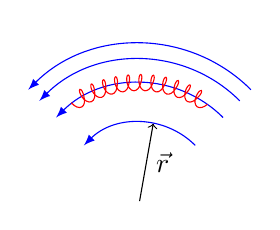
\begin{tikzpicture}[]
    \draw[->] (0,0) -- node[right] {$\vec{r}$} (80:1);
    \foreach \radius in {1,1.5,1.8,2} {
    \draw[-latex, blue] (45:\radius) arc[start angle=45, delta angle = 90, radius=\radius];
    }
    \draw[red, decoration={coil,amplitude=1mm,segment length=1.5mm}, decorate] (55:1.5) arc[start angle=55, delta angle = {2*(90-55)}, radius=1.5];
\end{tikzpicture}
		\end{column}
		\begin{column}{0.7\linewidth}
			Центр циклотронного кола рухатиметься по вздовж викривленої силової лінії. На нього діятиме відцентрова сила:
			\(
			\vec{F} = \dfrac{mv^2_\parallel}{r} \dfrac{\vec{r}}{r}.
			\)
		\end{column}
	\end{columns}
	\begin{block}{Швидкість відцентрового дрейфу}
		\begin{equation*}
			\tcbhighmath{
				\vec{v}_{cf} = \frac{v^2_\parallel}{\Omega r^2B}\left[ \vec{r}\times\vec{B}\right].
			}
		\end{equation*}
	\end{block}
	\begin{itemize}\justifying
		\item Якщо магнітне поле спрямоване до нас і випукле вгору, то позитивні частинки дрейфують праворуч, негативні --- ліворуч.
		\item Швидкість залежить від заряду частинки --- протилежно заряджені частинки дрейфують у протилежних напрямках, що  призводять до поділу зарядів.
	\end{itemize}
\end{frame}
% ===========================================================================




% ============================== Слайд ## ===================================
\begin{frame}{Відцентровий та градієнтний дрейфи}{}
	\begin{block}{}\justifying
		При викривлені ліній магнітного поля (в тороїдах) магнітне поле також має градієнт, тому \alert{поряд з відцентровим дрейфом відбувається і градієнтний дрейф}.
	\end{block}
	\begin{columns}
		\begin{column}{0.65\linewidth}
			В циліндричних координатах:
			\begin{equation*}
				B \sim \frac1r, \quad \nabla B \sim -\frac{\vec{r}}{r^2}, \quad \frac{\nabla B}{B} = -\frac{\vec{r}}{r^2}.
			\end{equation*}
		\end{column}
		\begin{column}{0.3\linewidth}
			\centering
			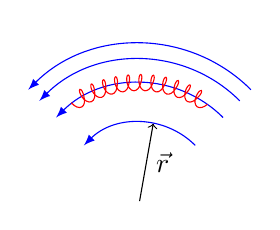
\begin{tikzpicture}[]
    \draw[->] (0,0) -- node[right] {$\vec{r}$} (80:1);
    \foreach \radius in {1,1.5,1.8,2} {
    \draw[-latex, blue] (45:\radius) arc[start angle=45, delta angle = 90, radius=\radius];
    }
    \draw[red, decoration={coil,amplitude=1mm,segment length=1.5mm}, decorate] (55:1.5) arc[start angle=55, delta angle = {2*(90-55)}, radius=1.5];
\end{tikzpicture}
		\end{column}
	\end{columns}
	Швидкість градієнтного дрейфу
	\(
	\vec{v}_{\nabla{B}} = \dfrac{v_\perp^2}2 \dfrac1{\Omega r^2}\dfrac{\vec{r}\times\vec{B}}{B}.
	\)

	\begin{block}{Сумарна швидкість дрейфу}
		\begin{equation*}
			\vec{v} = \vec{v}_{cf} + \vec{v}_{\nabla B}  = \frac{\left(v^2_\parallel + \frac12 v^2_\perp \right) }{\Omega r^2B}\left[ \vec{r}\times\vec{B}\right]
		\end{equation*}
	\end{block}
	\begin{alertblock}{}
		Швидкості обох дрейфів спрямовані в один бік.
	\end{alertblock}
\end{frame}
% ===========================================================================




%% --------------------------------------------------------
\section{Поляризаційний дрейф}
%% --------------------------------------------------------




% ============================== Слайд ## ===================================
\begin{frame}{Поляризаційний дрейф}{}\small
	\begin{block}{}\justifying
		За рахунок відцентрового і градієнтного дрейфів у плазмі тороїдальної пастки часто з'являються змінні електричні поля, що визначаються місцевим поділом зарядів, так звані поляризаційні поля. У цьому випадку на частинку діє змінна сила.
	\end{block}

	Рівняння руху:
	\begin{align*}
		\dot{v}_x & = \Omega v_y,                  \\
		\dot{v}_y & = -\Omega v_x + \frac{ZeE}{m}.
	\end{align*}

	Другі похідні:
	\begin{align*}
		\ddot{v}_x & = \Omega \dot{v}_y = -\Omega^2 v_x + \Omega^2 c\frac{E}{B},                                     \\
		\ddot{v}_y & = -\Omega \dot{v}_y + \frac{Ze\dot{E}}{m} = -\Omega^2 v_y + \Omega^2 c\frac{\dot{E}}{\Omega B}.
	\end{align*}
	Швидкість поляризаційного дрейфу
	\(
	\vec{v}_p = \dfrac{c}{\Omega B}\dfrac{\partial \vec{E}}{\partial t}.
	\)

\end{frame}
% ===========================================================================




%% --------------------------------------------------------
\section{Проблеми утримання плазми}
%% --------------------------------------------------------




% ============================== Слайд ## ===================================
\begin{frame}{Проблеми утримання плазми}{Тороїдальна камера}\small
	\begin{itemize}\justifying
		\item В тороїдальній камері лінії поля викривлені та існує градієнт поля до стінок, тому спостерігається як \alert{відцентровий} так і \alert{градієнтний} дрейфи частинок до стінок пастки, що призводить до розділення зарядів.

		      %			      {\tiny Градієнтний і відцентровий дрейфи спричиняють рух зарядів одного знака в один бік, а зарядів іншого знака в протилежний бік, унаслідок чого відбувається розподіл зарядів: вгорі камери утворюється надлишок негативних зарядів, а внизу --- позитивних.}

		\item Розділення зарядів призводить до появи електричного поля, яке перпендикулярне до магнітного поля. А електричне поле, що виникло, викликає \alert{електричний} дрейф частинок, і плазма як ціле спрямовується до стінки і <<гине>> на цьому етапі.
	\end{itemize}
	\begin{center}
		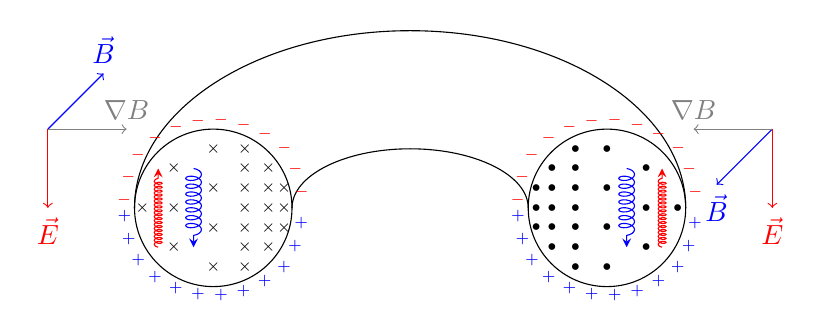
\begin{tikzpicture}
    \draw (-2.5, 0) circle (1);
    \draw (2.5, 0) circle (1);

    \draw (3.5, 0) arc[start angle=0, end angle=180, x radius = 3.5, y radius = 2.25];
    \draw (1.5, 0) arc[start angle=0, end angle=180, x radius = 1.5, y radius = 0.75];
    \foreach \i/\mf in {1/$\times$, -1/$\bullet$} {
    \begin{scope}[xscale=\i]
     \foreach \y in {-0.25,0,...,0.25} {
                \node[font=\tiny] at (-1.6, \y) {\mf};
        }
        \foreach \y in {-0.5,-0.25,...,0.5} {
            \node[font=\tiny] at (-1.8, \y) {\mf};
        }
        \foreach \y in {-0.75,-0.5,...,0.75} {
                \node[font=\tiny] at (-2.1, \y) {\mf};
        }
        \foreach \y in {-0.75,-0.25,...,0.75} {
                \node[font=\tiny] at (-2.5, \y) {\mf};
        }
        \foreach \y in {-0.5,0,...,0.5} {
                \node[font=\tiny] at (-3, \y) {\mf};
        }
        \node[font=\tiny] at (-3.4, 0) {\mf};
    \end{scope}
    }

    \foreach \i in {1, -1} {
    \begin{scope}[xscale=\i]
        \draw[-stealth, red, decoration={
        coil,
        amplitude=0.5mm,
        segment length=0.5mm,
        post length=3pt
        },
        decorate] (-3.2, -0.5) -- ++(0, 1);
        \draw[-stealth, blue, decoration={
        coil,
        amplitude=1mm,
        segment length=1mm,
        post length=2pt
        }, decorate] (-2.75, 0.5) -- ++(0, -1);

       \begin{scope}[yshift=1cm]
        \draw[->, blue, yscale=\i] (-4.6, 0) -- ++(45:1) node[anchor={-\i*90}] {$\vec{B}$};

        \draw[->, red] (-4.6, 0) -- ++(0, -1) node[anchor=north] {$\vec{E}$};

        \draw[->, gray, yscale=\i] (-4.6, 0) -- ++(1, 0) node[anchor=south] {$\nabla{B}$};
       \end{scope}
    \end{scope}


    \foreach \a in {10,25,...,180} {
            \node[xshift={\i*2.5cm}, font=\tiny, anchor={180+\a}, inner sep=1pt, text=red] at (\a:1) {$-$};
            \node[xshift={\i*2.5cm}, font=\tiny, anchor={180-\a}, inner sep=1pt, text=blue] at (-\a:1) {$+$};
            }
        }
\end{tikzpicture}
	\end{center}
\end{frame}
% ===========================================================================



% ============================== Слайд ## ===================================
\begin{frame}{Задачі}{}
	\begin{onlyenv}<1>
		\begin{exampleblock}{Задача 1}% Чен 2.1
			\justifying
			Обчисліть ларморівський радіус у таких випадках:
			\begin{enumerate}
				\item для електрона з енергією $10$~кеВ, що перебуває в магнітному полі Землі.
				\item для протона з потоку сонячного вітру, швидкість руху якого в
				      міжпланетному магнітному полі $B = 5\cdot10^{-9}$~Тл становить $300$ км/с;
				\item  для іона \ce{He^+} з енергією $1$~кеВ, що перебуває в атмосфері Сонця поблизу плями, де $B = 5\cdot10^{-2}$~Тл;
				\item для частинки домішки \ce{He^{++}} з енергією $3.5$~МеВ у дейтерієво-тритієвому реакторі синтезу з магнітним полем $B = 8$~Тл.
			\end{enumerate}
		\end{exampleblock}
		\begin{exampleblock}{Задача 2}% Котельников
			\justifying
			Знайдіть швидкість руху та траєкторію частинки якщо $\vec{E}\parallel\vec{B}$ та електричне поля паралельні.
		\end{exampleblock}
	\end{onlyenv}
	\begin{onlyenv}<2>
		\begin{exampleblock}{Задача 3}% Козел 3.137
			\justifying
			У схрещених однорідних полях $Е_у$ і $B_z$ з деякої точки $x_0$ розлітаються електрони з однаковими швидкостями $v \ll c$, що лежать у площині $xy$. Вважаючи $Е_у \ll B_z$ і нехтуючи взаємодією електронів один з одним, знайти, на якій відстані $\ell$ і через який час $t$ вони знову зберуться в одну точку.
		\end{exampleblock}
		\begin{exampleblock}{Задача 4}% Чен 2.3
			\justifying
			В іонному двигуні створюється магнітне поле величиною $1$~Тл, а воднева плазма внаслідок електричного дрейфу виштовхується з нього зі швидкістю $1000$~км/с. Наскільки великим має бути для цього електричне поле всередині плазми?
		\end{exampleblock}
	\end{onlyenv}
    \begin{onlyenv}<3>
            \begin{exampleblock}{Задача 5}\justifying%Чен 2.8
                Припустимо, що магнітне поле Землі на екваторі дорівнює $3\cdot10^{-5}$~Тл і спадає з відстанню за законом $\sim \frac{1}{r^3}$ (як у диполя).
                Нехай на відстані $r = 5R_\text{З}$ від центру Землі в екваторіальній площині є ізотропні розподіли протонів з енергією $1$~еВ і електронів з енергією $30$~кеВ, густиною $n = 10^7$~м\textsuperscript{-3} кожне.
                \begin{enumerate}
                    \item Обчисліть швидкості градієнтних дрейфів іонів та електронів.
                    \item На захід чи на схід дрейфують електрони?
                    \item Скільки часу знадобиться електрону, щоб обійти навколо Землі?
                    \item Обчисліть густину кільцевого струму, що виникає через дрейф.
                \end{enumerate}
        \end{exampleblock}
    \end{onlyenv}
\end{frame}
% ===========================================================================

\end{document}

